\documentclass[a4paper]{article}
\usepackage[italian]{babel}
\usepackage[italian]{isodate}  		% formato delle date in italiano
\usepackage{graphicx}				% gestione delle immagini
\usepackage{amsfonts}
\usepackage{booktabs}				% tabelle di qualità superiore
\usepackage{amsmath}				% pacchetto matematica
\usepackage{mathtools}				% per sottolineare sotto le equazioni
\usepackage{enumitem}				% gestione delle liste
\usepackage{pifont}					% pacchetto con elenchi carini
\usepackage[x11names]{xcolor}		% colori aggiuntivi
% Link ipertestuali per l'indice
\usepackage{xcolor}
\usepackage[linkcolor=black, citecolor=blue, urlcolor=cyan]{hyperref}
\hypersetup{
	colorlinks=true
}

%\usepackage{showframe}				% visualizzazione bordi
%\usepackage{showkeys}				% visualizzazione etichetta

\newtheorem{theorem}{Teorema}
\newcommand{\dquotes}[1]{``#1''}

\begin{document}
	\author{VR443470}
	\title{Analisi II}
	\date{\printdayoff\today}
	\maketitle
	
	\newpage
	
	% indice
	\tableofcontents
	
	\newpage
	
	%%%%%%%%%%%%%%
	% LEZIONE 01 %
	%%%%%%%%%%%%%%
	\section{Lezione 01}
	
	\subsection{Equazioni a variabili separabili}\label{Equazioni a variabili separabili}
	
	Le equazioni differenziali a \textbf{variabili separabili} hanno due forme:
	
	\begin{itemize}
		\item \textbf{Forma canonica.} $y'(x) = f(x)\cdot g\left(y(x)\right)$
		\item \textbf{Forma alternativa.} $y' = f(x) \cdot g(y)$
	\end{itemize}
	
	\noindent
	Dove $f$ e $g$ sono funzioni continue ``in un intervallo reale'', più formalmente:
	
	\begin{gather*}
		f \text{ continua in } I \subseteq R \\
		g \text{ continua in } J \subseteq R
	\end{gather*}
	
	\noindent
	Le \textcolor{Red3}{\textbf{soluzioni}} di un'equazione differenziale possono essere:
	
	\begin{itemize}
		\item[\ding{51}] \textbf{Costanti.} Quando $\bar{y}\in\mathbb{R}$ è uno zero di $g(y)$ e dunque vale:
		\begin{equation*}
			y(x)=\bar{y} \hspace{1em} \forall x\in I
		\end{equation*}

		\noindent
		Quindi, quando un valore annulla $g(y)$, vuol dire che è stata trovata una soluzione costante dell'equazione differenziale.
		
		\item[\ding{51}] \textbf{\underline{Non} costanti.} Quando $g(y)$ non si annulla e quindi ci sarà la relazione:
		\begin{equation*}
			y'(x) = f(x) \cdot g(y(x)) \longrightarrow \dfrac{y'(x)}{g(y(x))} = f(x)
		\end{equation*}
	\end{itemize}

	\noindent
	Tuttavia, supponendo che $G(y)$ sia una primitiva di $\dfrac{1}{g(y)}$, allora:
	
	\begin{equation*}
		\dfrac{\mathrm{d}}{\mathrm{d}x} G\left(y(x)\right) = f(x) \hspace{2em} \text{con} \hspace{2em} G(x) = F(x) + c \hspace{1em} c\in\mathbb{R}
	\end{equation*}
	
	\noindent
	Dove $F(x)$ è la primitiva di $f(x)$. Ma dato che $G$ è invertibile, si scrive:
	
	\begin{equation}\label{integrale_generale}
		y(x) = G^{-1} \left(F(x) + c\right) \hspace{2em} \text{con } c \in \mathbb{R}
	\end{equation}

	\noindent
	L'equazione \ref{integrale_generale} rappresenta l'\textbf{insieme delle soluzioni dell'equazione differenziale} e viene chiamato anche \textcolor{Red3}{\textbf{integrale generale}}.
	
	\newpage
	
	\begin{center}
		\large \textcolor{Green4}{\textbf{Esempio equazione differenziale a variabili separabili}}
	\end{center}
	
	\noindent
	Equazione differenziale: $y' = x y$ in cui la $x$ rappresenta $f(x)$ e la $y$ rappresenta la $g(y)$. Una \textbf{nuova notazione} utilizzata negli esercizi è la seguente:
	
	\begin{equation*}
		f, g \in \mathcal{C}^{0}(\mathbb{R})
	\end{equation*}

	\noindent
	Che indica che le \textbf{funzioni $f$ e $g$ sono continue nell'intervallo $\mathbb{R}$}.
	
	L'esercizio si svolge \emph{cercando} inizialmente le \underline{soluzioni costanti}. Il modo più semplice per farlo è porre $y=0$ e verificare se $g(y)$ si annulla: in caso affermativo esiste una soluzione costante. In questo esercizio si annulla, quindi \emph{ha soluzione costante}.
	
	Al contrario, le \underline{soluzioni \emph{non} costanti} si trovano quando $y \ne 0$. Quindi:
	
	\begin{gather*}
		y' = xy \rightarrow \dfrac{\mathrm{d}y}{\mathrm{d}x} = xy \rightarrow \dfrac{1}{y} \mathrm{d}y = x \: \mathrm{d}x \rightarrow \displaystyle \int \dfrac{1}{y} \mathrm{d}y = \int x \mathrm{d} x \rightarrow \ln |y| = \dfrac{1}{2} x^{2} + c \hspace{1em} c\in\mathbb{R}
	\end{gather*}

	\noindent
	Esplicitando il risultato:
	
	\begin{equation*}
		|y(x)| = e^{\frac{1}{2} x^2 + c} \hspace{1em} c\in\mathbb{R} \longrightarrow y(x) = \pm e^{c} \cdot e^{\frac{1}{2} x^2} \hspace{1em} c \in \mathbb{R}
	\end{equation*}

	Dato che $e^c$ può essere positivo o negativo escluso lo zero (soluzione costante!), si riscrive più precisamente l'\textbf{integrale generale dell'equazione}:
	
	\begin{equation*}
		y(x) = k \cdot e^{\frac{1}{2} x^2} \hspace{1em} k \in \mathbb{R} \setminus \{0\}
	\end{equation*}

	È possibile \textbf{verificare la soluzione} dell'equazione differenziale effettuando una derivazione:
	
	\begin{gather*}
		y(x) = k \cdot e^{\frac{1}{2} x^2} \\
		y'(x) = k \cdot x \cdot e^{\frac{1}{2} x^2} \hspace{1em} \forall x \in \mathbb{R} \hspace{1em} \text{\textcolor{Green3}{\checkmark Verificata}}
	\end{gather*}
	
	\newpage
	
	\subsection{Problema di Cauchy}
	
	Nel caso in cui si è interessati ad una soluzione particolare, è necessaria una condizione. In questo caso, si è di fronte al \textcolor{Red3}{\textbf{problema di Cauchy}}, il quale è caratterizzato dalla presenza di un'equazione differenziale e da \underline{almeno} una condizione.\newline
	L'\textbf{obbiettivo} è \underline{verificare} la/le condizione/i tramite una soluzione (o più soluzioni).\newline
	La \textbf{struttura} è la seguente:
	
	\begin{equation}\label{problema_di_Cauchy}
		\begin{cases}
			y'= f(x) \cdot g(y) \\
			y(x_0) = y_0 & x_0 \in I
		\end{cases}
	\end{equation}

	\vspace{1em}

	\begin{center}
		\large \textcolor{Green4}{\textbf{Esempio problema di Cauchy}}
	\end{center}

	\noindent
	Il problema:
	
	\begin{equation*}
		\begin{cases}
			y' = -3y \\
			y(0) = 2
		\end{cases}
	\end{equation*}

	\noindent
	La risoluzione:
	
	\begin{gather*}
		\dfrac{\mathrm{d}y}{\mathrm{d}x} = - 3y \longrightarrow \dfrac{\mathrm{d}y}{y} = - 3 \: \mathrm{d}x \longrightarrow  \displaystyle \int {\dfrac{1}{y} \: \mathrm{d}y} = -3x + c \longrightarrow ...\\
		... \longrightarrow y(x) = k e^{-3x} \hspace{1em} k \in \mathbb{R} \text{ [}\textcolor{Red3}{\textbf{Integrale generale}}\text{]}
	\end{gather*}

	\noindent
	Adesso si esegue la \textbf{verifica della condizione} sostituendo quest'ultima nella soluzione:
	
	\begin{gather*}
		\text{Condizione: } y(0) = 2 \\
		\text{Eq. diff.: } y(0) = k e^{-3 \cdot (0)} \longrightarrow 2 = k \cdot e^0 \longrightarrow k = 2
	\end{gather*}

	\noindent
	Quindi, la \textbf{soluzione del problema di Cauchy}:
	
	\begin{equation*}
		y(x) = 2 e^{-3x} \hspace{1em} \text{con } x \in \mathbb{R}
	\end{equation*}

	\newpage
	
	\begin{center}
		\large \textcolor{Green4}{\textbf{Un altro esempio del problema di Cauchy}}
	\end{center}

	\noindent
	Il problema:
	
	\begin{equation*}
		\begin{cases}
			y' = (1 + y^2) x & f, g \in \mathcal{C}^0 \left(\mathbb{R}\right) \\
			y(0) = 1
		\end{cases}
	\end{equation*}

	\noindent
	Cercando la \textbf{soluzione costante} sostituendo $y = 0$, si osserva che la funzione non si annulla, quindi $1 + y^2 \ne 0 \hspace{1em} \forall y \in \mathbb{R}$, ovvero nessun numero reale annulla $g(y)$.
	
	\noindent
	Cercando eventuali \textbf{soluzioni costanti}:
	
	\begin{gather*}
		\dfrac{\mathrm{d}y}{\mathrm{d}x} = (1 + y^2) x \longrightarrow \dfrac{1}{1 + y^2} \mathrm{d}y = x \mathrm{d}x \longrightarrow \int{\dfrac{1}{1 + y^2} \mathrm{d}y} = \int{x \mathrm{d}x} \longrightarrow \\
		\longrightarrow \textcolor{Red3}{\textbf{ Integrale generale}}\text{: } \arctan{\left(y\right)} = \dfrac{1}{2} x^2 + c \hspace{1em} c \in \mathbb{R}
	\end{gather*}

	\noindent
	\textbf{Verificando la condizione} sostituendo, si ottiene:
	
	\begin{gather*}
		\text{Condizione: } y(0) = 1 \\
		\text{Eq. diff.: } \arctan{\left(1\right)} = \dfrac{1}{2}\cdot 0^2 + c \longrightarrow \arctan{\left(1\right)} = 0 + c \longrightarrow c = \dfrac{\pi}{4}
	\end{gather*}
	
	\noindent
	È possibile \textbf{esplicitare} la funzione $y(x)$ dall'integrale generale, ottenendo la seguente forma:
	
	\begin{equation*}
		y(x) = \tan{\left(\dfrac{1}{2}x^2 + \dfrac{\pi}{4}\right)}
	\end{equation*}

	\noindent
	Inoltre, dato che $\arctan$ è sicuramente compreso, per definizione, nell'intervallo:
	
	\begin{equation*}
		\pm \dfrac{\pi}{2} \longrightarrow -\dfrac{\pi}{2} < \dfrac{1}{2} x^2 + c < \dfrac{\pi}{2}
	\end{equation*}

	\noindent
	Allora è possibile sostituire la $c$ con il valore trovato durante l'esplicitazione:s
	
	\begin{equation*}
		-\dfrac{\pi}{2} < \dfrac{1}{2} x^2 + \dfrac{\pi}{4} < \dfrac{\pi}{2}
	\end{equation*}

	\noindent
	Per controllare che la soluzione sia effettivamente all'\textbf{interno dell'intervallo}, avviene nel seguente modo:
	
	\begin{equation*}
		-\dfrac{\pi}{2} < \dfrac{1}{2} x^2 + \dfrac{\pi}{4} < + \dfrac{\pi}{2}
	\end{equation*}

	\noindent
	Sicuramente $-\dfrac{\pi}{2} < \dfrac{1}{2} x^2 + \dfrac{\pi}{4}$ è verificata per $x \in \mathbb{R}$. La parte di destra è possibile verificarla effettuando qualche manipolazione sulla disuguaglianza:
	
	\begin{equation*}
		\dfrac{1}{2} x^2 + \dfrac{\pi}{4} < + \dfrac{\pi}{2} \longrightarrow \dfrac{1}{2} x^2 < \dfrac{\pi}{2} - \dfrac{\pi}{4} \longrightarrow \dfrac{1}{2} x^2 < \dfrac{\pi}{4} \longrightarrow x^2 < \dfrac{\pi}{2}
	\end{equation*}

	\noindent
	Quindi, la soluzione è corretta quando $x$ è nell'intervallo (esplicitando):
	
	\begin{equation*}
		- \sqrt{\dfrac{\pi}{2}} < x < + \sqrt{\dfrac{\pi}{2}}
	\end{equation*}

	\newpage

	\noindent
	Quindi, l'\textcolor{Red3}{\textbf{intervallo massimale delle soluzioni}}, ovvero il più grande intervallo in cui è definita la soluzione del problema di Cauchy, è così definita:
	
	\begin{figure}[!htp]
		\centering
		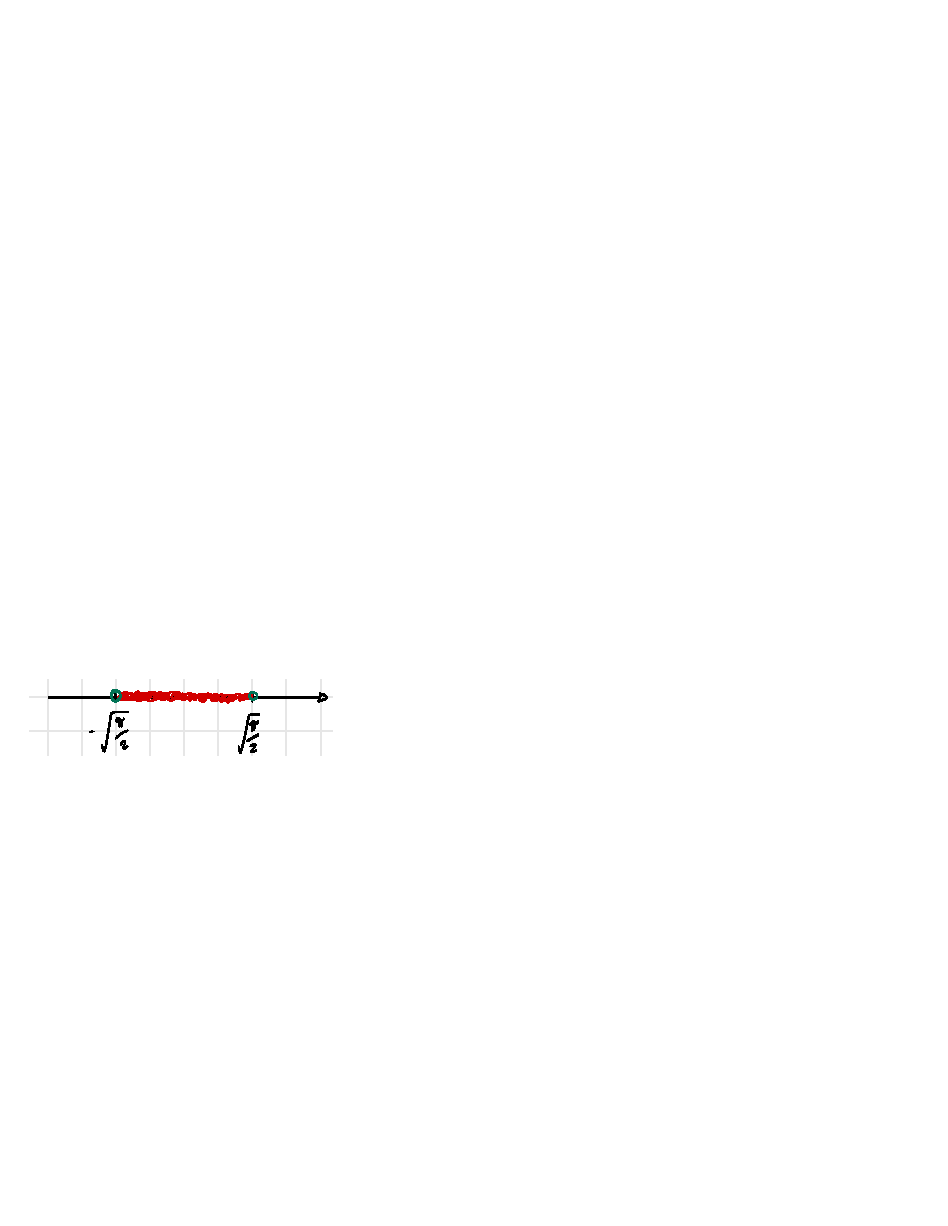
\includegraphics[width=0.7\textwidth]{img/intervallo_max_eg.pdf}
		\caption{Intervallo massimale delle soluzioni.}
	\end{figure}

	\newpage

	%%%%%%%%%%%%%%
	% LEZIONE 02 %
	%%%%%%%%%%%%%%
	\section{Lezione 02}
	
	\subsection[Problema di Cauchy per eq. diff. a variabili separabili]{Problema di Cauchy per equazioni differenziali a variabili separabili}
	
	Per introdurre il problema di Cauchy con le equazioni differenziali a variabili separabili, è necessario introdurre il \textbf{teorema di \underline{esistenza} e \underline{unicità}}.\newline
	
	\noindent
	Si consideri il problema:
	
	\begin{equation*}
		\begin{cases}
			y^{'} = f\left(x\right) \cdot g\left(y\right) \\
			y\left(x_{0}\right) = y_{0}
		\end{cases}
	\end{equation*}

	\noindent
	In cui $f$ è una funzione continua su $I = \left(x_{0} - r_{1}, x_{0} + r_{1}\right)$ e $g$ è una funzione continua su un intervallo $J = \left(y_{0} - r_{2}, y_{0} + r_{2}\right)$.
	
	\begin{theorem}[Esistenza]\label{teorema esistenza}
		Esiste una soluzione al problema di Cauchy definita per ogni $x \in I^{'} = \left[x_{0} - \delta, x + \delta\right] \subseteq I$. È dunque \textbf{garantita la soluzione locale} e non obbligatoriamente su tutto l'intervallo $I$.
	\end{theorem}

	\begin{theorem}[Unicità]\label{teorema unicità}
		Se $g\left(y\right)$ è \underline{continua e derivabile} con derivata continua (formalmente: $g\left(y\right) \in \mathcal{C}^{1} \left(J\right)$), allora la \textbf{soluzione è unica}.
	\end{theorem}

	\begin{figure}[!htp]
		\centering
		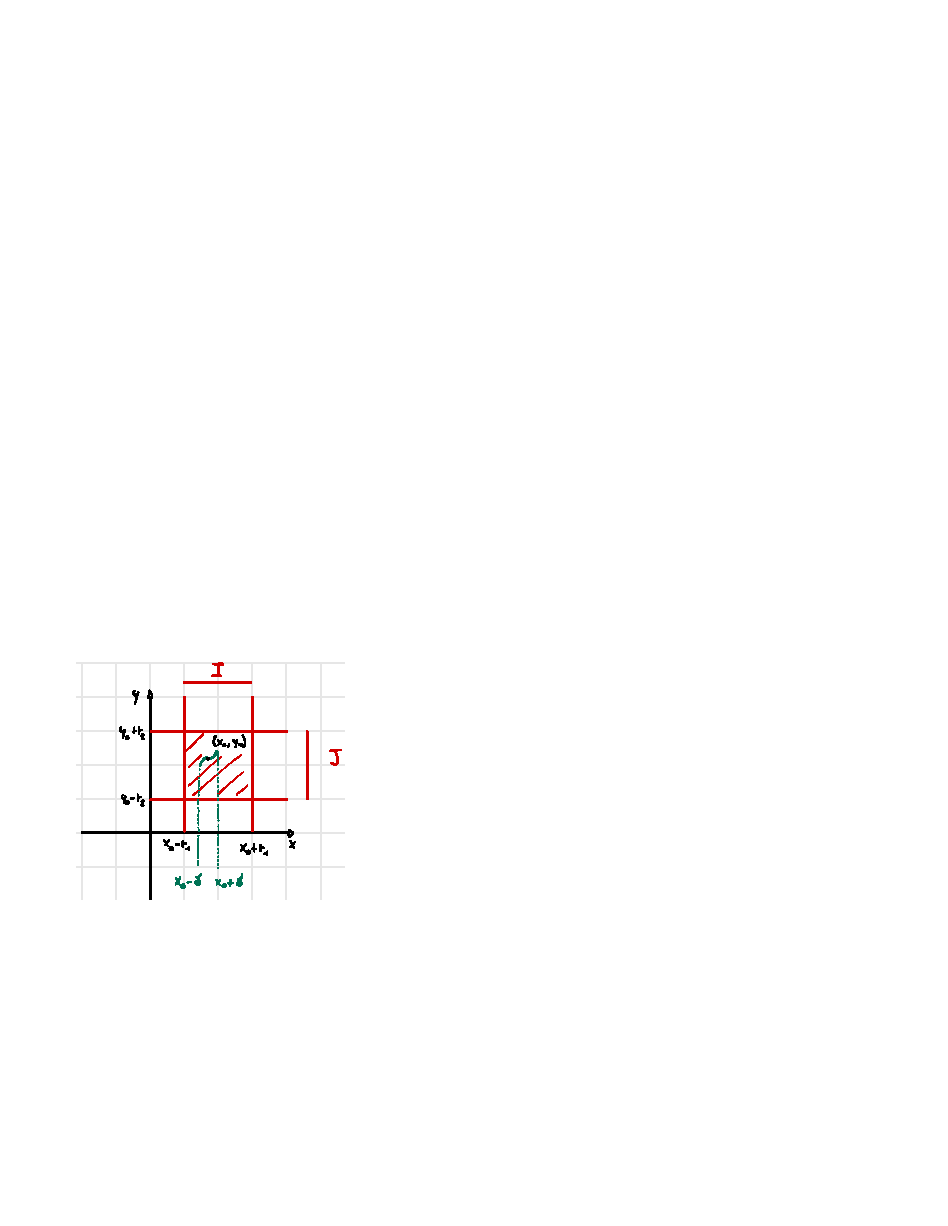
\includegraphics[width=0.8\textwidth]{img/prob_cauchy-variabili_separabili.pdf}
		\caption{Rappresentazione grafica del problema di Cauchy con variabili separabili.}
	\end{figure}

	\newpage

	\noindent
	\textbf{Caso in cui il teorema dell'unicità viene violato! È facilmente riconoscibile poiché ci sono due soluzioni che passano per la condizione imposta $\left(\text{il punto } x_{0}, y_{0}\right)$.}
	
	\begin{figure}[!htp]
		\centering
		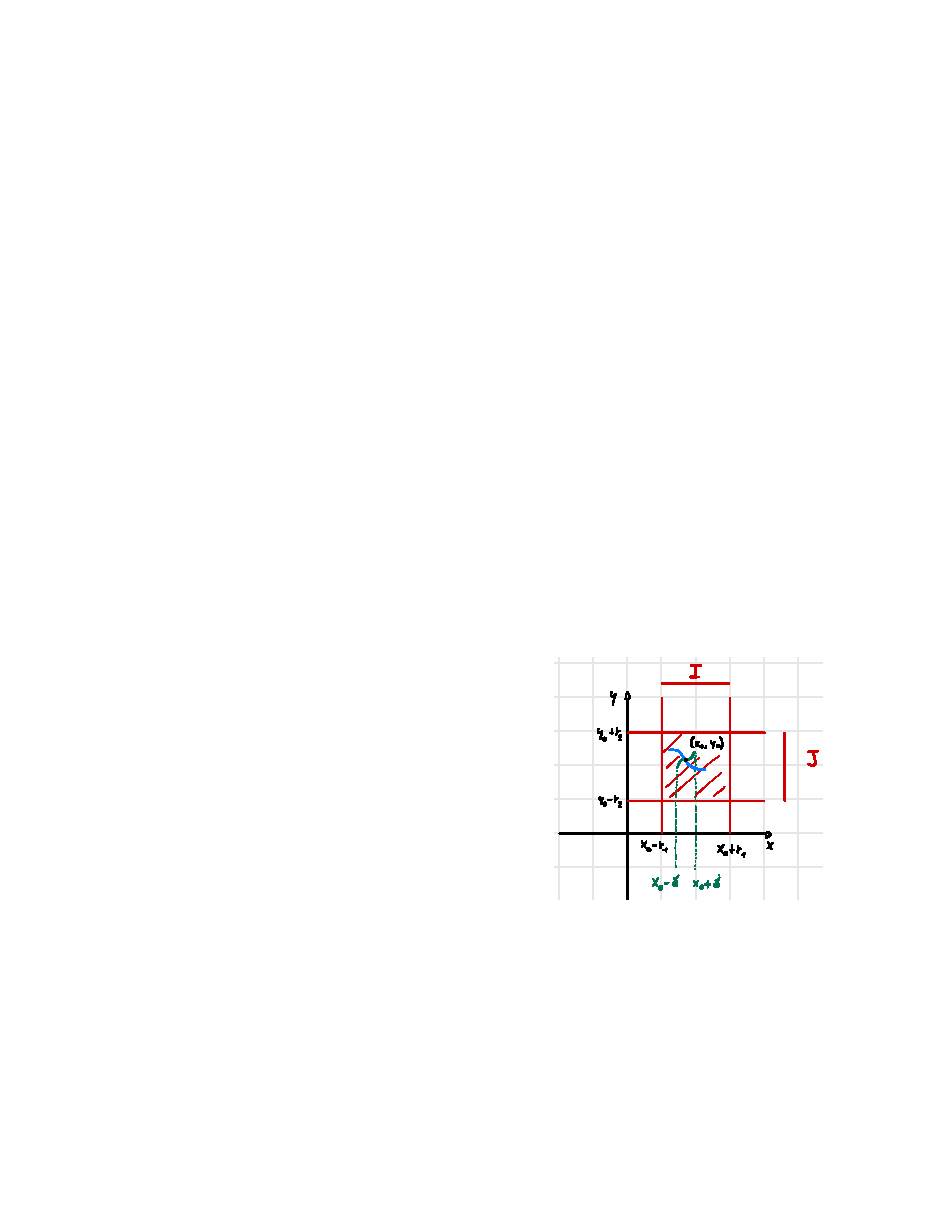
\includegraphics[width=0.8\textwidth]{img/prob_cauchy-variabili_separabili_violazione.pdf}
		\caption{Teorema dell'esistenza garantito, ma teorema dell'unicità violato.}
	\end{figure}

	\newpage
	
	\subsection{Esempi di problemi di Cauchy}
	
	\subsubsection[Esempio semplice]{\textcolor{Green4}{\textbf{Esempio semplice}}}
	
	\noindent
	Il problema:
	
	\begin{equation*}
		\begin{cases}
			y' \cdot y = 1 \\
			y\left(1\right) = 0
		\end{cases}
	\end{equation*}
	
	\noindent
	In questo caso \textbf{\underline{non esiste una soluzione}} poiché $y^{'}\left(1\right) \cdot y\left(1\right)$ deve essere uguale a $1$. Se nell'espressione $y^{'}\left(1\right) \cdot y\left(1\right) = 1$ vengono sostituite le funzioni con il valore zero, risulta impossibile l'uguaglianza: $y^{'}\left(1\right) \cdot 0 = 1$.\newline
	
	\subsubsection[Esempio medio]{\textcolor{Green4}{\textbf{Esempio medio}}}
	
	\noindent
	Il problema:
	
	\begin{equation*}
		\begin{cases}
			y' = y^{\frac{2}{3}} \\
			y\left(0\right) = 0
		\end{cases}
	\end{equation*}
	
	\noindent
	Esiste sicuramente \textbf{\underline{una soluzione costante}} con $y = 0$.
	
	Inoltre, andando a studiare le \textbf{\underline{soluzioni non costanti}}, quindi con $y \ne 0$, si evince chiaramente che:
	
	\begin{gather*}
		y^{'} = y^{\frac{2}{3}} \longrightarrow
		\dfrac{\mathrm{d}y}{y^{\frac{2}{3}}} = \mathrm{d}x \longrightarrow
		y^{-\frac{2}{3}} \mathrm{d}y = \mathrm{d}x \\
		\textbf{Integrando...} \longrightarrow
		3y^{\frac{1}{3}} = x + c
	\end{gather*}

	\noindent
	Dato che utilizzando la condizione del problema $y\left(0\right) = 0$ la $c$ è zero:
	
	\begin{equation*}
		3\left(y\left(0\right)^{\frac{1}{3}}\right) = 0 + c
	\end{equation*}

	\noindent
	Esplicitando la $y$, si ottiene la \textbf{soluzione al problema di Cauchy}:
	
	\begin{equation*}
		y = \dfrac{1}{27} x^{3} \hspace{2em} \text{con } x \ge 0
	\end{equation*}

	\newpage

	\noindent\fbox{%
		\parbox{\textwidth}{%
			È interessante notare che la soluzione può essere prolungata a tutto l'insieme dei reali $\mathbb{R}$:
			
			\begin{equation*}
				\tilde{y}\left(x\right) = 
				\begin{cases}
					0 					& x < 0 \\
					\dfrac{1}{27} x^{3} & x \ge 0
				\end{cases}
			\end{equation*}
		
			\noindent
			Inoltre, è possibile anche traslare funzioni di questo tipo:
			
			\begin{equation*}
				\tilde{y}\left(x\right) = 
				\begin{cases}
					0 & x < \alpha \\
					\dfrac{1}{27} \left(x - \alpha\right)^{3} & x \ge \alpha
				\end{cases}
			\end{equation*}
			
			\noindent
			Questo dimostra che la funzione ha una derivata non limitata nell'intervallo.
		}%
	}

	\begin{figure}[!htp]
		\centering
		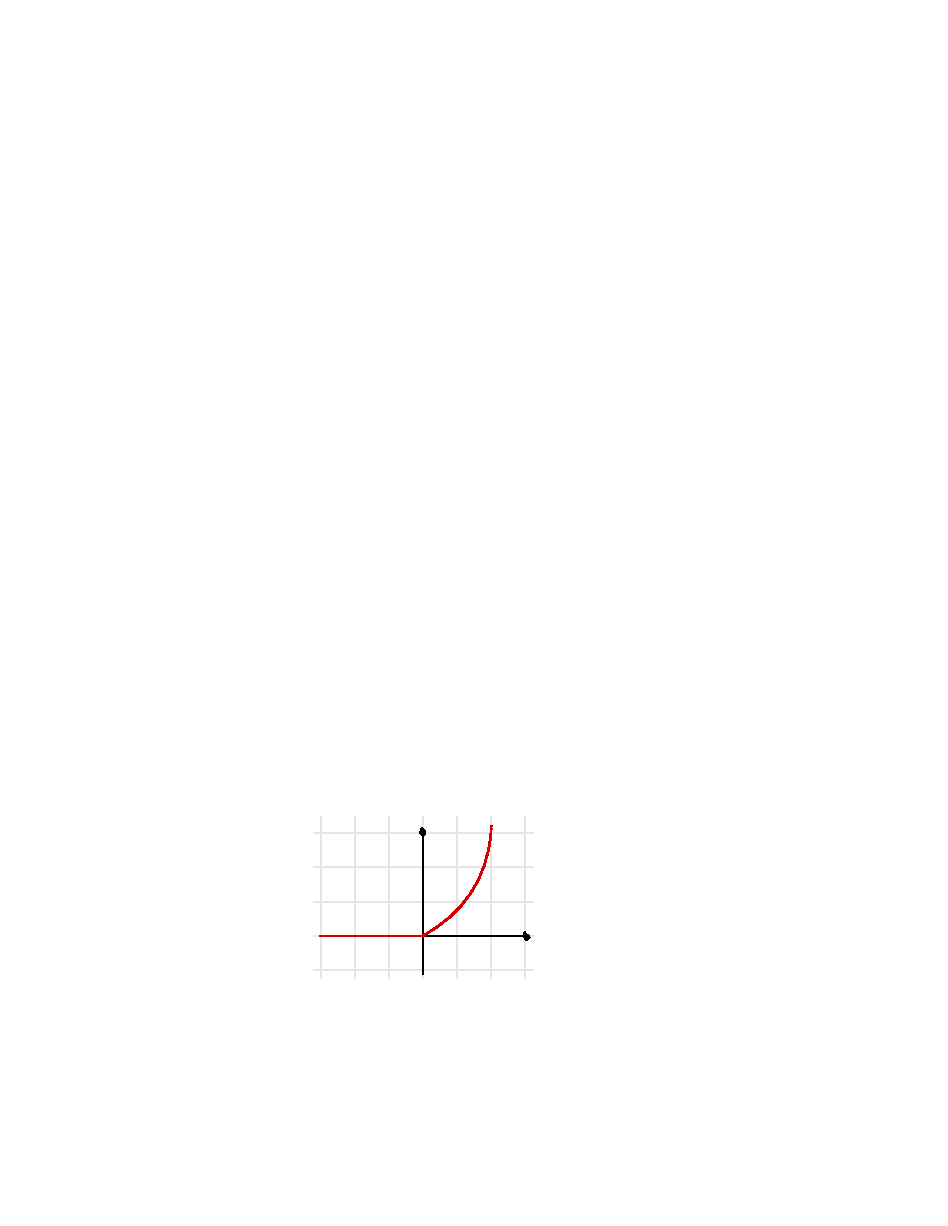
\includegraphics[width=0.6\textwidth]{img/prob_cauchy-variabili_separabili-OSS.pdf}
		\caption{Grafico dell'osservazione estesa a $\mathbb{R}$.}
		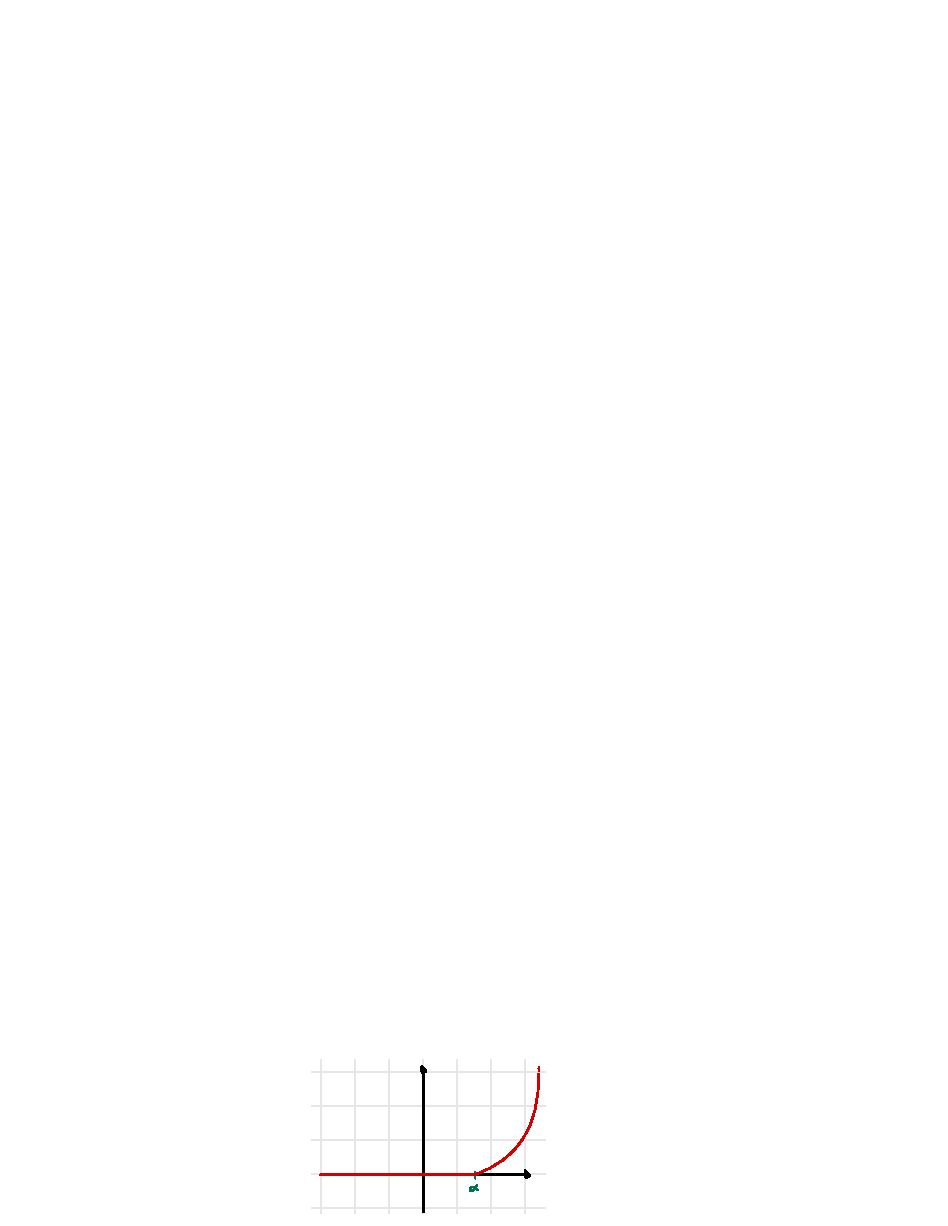
\includegraphics[width=0.6\textwidth]{img/prob_cauchy-variabili_separabili-OSS2.pdf}
		\caption{Grafico dell'osservazione estesa a $\mathbb{R}$ e traslata di $\alpha$.}
	\end{figure}

	\newpage
	
	\subsubsection[Esempio difficile]{\textcolor{Green4}{\textbf{Esempio difficile}}}
	
	\noindent
	Il problema:
	
	\begin{equation*}
		\begin{cases}
			e^{x+y} \cdot y + x = 0 \\
			y\left(0\right) = 0
		\end{cases}
	\end{equation*}
	
	\noindent
	Tuttavia, la funzione non è in forma canonica, quindi si eseguono alcune operazioni algebriche:
	
	\begin{equation*}
		e^{x+y} \cdot y + x = 0 \longrightarrow e^{x+y} \cdot y = -x \longrightarrow y^{'} = - \dfrac{x}{e^{x+y}}
	\end{equation*}

	\noindent
	Quindi:
	
	\begin{equation*}
		\begin{cases}
			y^{'} = - \dfrac{x}{e^{x+y}} \\
			y\left(0\right) = 0
		\end{cases}
	\end{equation*}

	\noindent
	Il problema si risolve tramite la \textbf{\underline{tecnica delle variabili separabili}}. Infatti:
	\begin{equation*}
		y^{'} = -\dfrac{x}{e^{x+y}}; \hspace{1em}
		y^{'} = -\dfrac{x}{e^{x} \cdot e^{y}}; \hspace{1em}
		y^{'} = -\dfrac{x}{e^{x}} \cdot \dfrac{1}{e^{y}}; \hspace{1em}
		y^{'} = - \underbracket[0.14ex]{x \cdot e^{-x}}_{f\left(x\right)} \cdot \underbracket[0.14ex]{e^{-y}}_{g\left(y\right)}
	\end{equation*}

	\noindent
	Con gli intervalli definiti in tutto $\mathbb{R}$ cioè $I = J = \mathbb{R}$.
	
	\noindent
	La risoluzione si svolge separando le variabili e integrando (N.B. la funzione $g\left(y\right)$ non ha zeri e quindi \textbf{\underline{non esistono soluzioni costanti}}):
	
	\begin{gather*}
		e^{y} \mathrm{d}y = -x e^{-x} \mathrm{d}x; \hspace{1em}
		\int e^{y} \mathrm{d}y = \int -x e{-x} \mathrm{d}x; \hspace{1em}
		e^{y} = x e^{-x} - \int 1 \cdot e^{-x} \mathrm{d}x; \hspace{1em} \\
		\textbf{Soluzione: } e^{y} = x e^{-x} + e^{-x} + c
	\end{gather*}

	\noindent
	Dunque, l'\textbf{\underline{integrale generale}}:
	
	\begin{equation*}
		y\left(x\right) = \ln \left(x e^{-x} + e^{-x} + c\right)
	\end{equation*}

	\noindent
	Imponendo la \textbf{condizione iniziale}:
	
	\begin{equation*}
		y\left(0\right) = \ln \left(1+c\right) \hspace{2em} \text{con } c = 0
	\end{equation*}

	\noindent
	Per cui, la \textbf{\underline{soluzione al problema di Cauchy}} è:
	
	\begin{equation*}
		y\left(x\right) = \ln\left(x e^{-x} + e^{-x}\right) \hspace{2em} \text{con } x > -1
	\end{equation*}

	\noindent
	L'\textbf{\underline{intervallo massimale}} è:
	
	\begin{equation*}
		\left(-1; +\infty\right)
	\end{equation*}

	\newpage
	
	\subsection{Modello di crescita logaritmica}
	
	Creato dal matematico belga Verhulst, riguarda le equazioni differenziali. Infatti, la forma generale trovata nei problemi di Cauchy è del tipo $y^{'} = a y \left(1 - by\right)$, ma in questo modello è importante una forma alternativa della funzione del problema di Cauchy:
	
	\begin{equation*}
		\begin{cases}
			\text{Funzione:} & y^{'} = k y \left(1 - y\right) \\
			\text{Condizione:} & y\left(0\right) = y_{0}
		\end{cases}
	\end{equation*}

	\noindent
	In modo più formale, nel modello di crescita logaritmica l'equazione differenziale rappresenta una frazione di popolazione. Dunque, è possibile riscriverla come:
	
	\begin{equation*}
		\begin{cases}
			y^{'} = k y\left(1 - y\right) & 0 \le y \le 1 \\
			y\left(0\right) = y_{0} & \text{altrimenti}
		\end{cases}
	\end{equation*}

	\noindent
	In questo caso, le \textbf{\underline{soluzioni costanti} (o stabili, o d'equilibrio)} sono $y = 0$ e $y = 1$. Invece, le \textbf{\underline{soluzioni \emph{non} costanti}} sono:
	
	\begin{gather*}
		\dfrac{\mathrm{d}y}{y\left(1 - y\right)} = k \mathrm{d}x \xlongrightarrow{\text{Integrando...}}
		\int \dfrac{\mathrm{d}y}{y\left(1 - y\right)} = \int k \mathrm{d}x; \\
		\ln\left(y\right) - \ln\left(1 - y\right) = k x + c; \\
		\ln\left(\dfrac{y}{1 - y}\right) = k x + c
	\end{gather*}

	\noindent
	Nonostante la forma sia corretta, è utile avere la $y$ esplicitata, quindi:
	
	\begin{gather*}
		\begin{matrix}
			\dfrac{y}{1 - y} = e^{kx} \cdot e^{c}; & y = e^{c} \cdot e^{kx} \cdot \left(1 - y\right); \\
			\\
			y = e^{c} \cdot e^{kx} - e^{c} \cdot e^{kx} y; & y\left(1 + e^{c} \cdot e^{kx}\right) = e^{c} \cdot e^{kx}; \\
			\\
			y\left(x\right) = \dfrac{e^{c} \cdot e^{kx}}{1 + e^{c} \cdot e^{kx}}
		\end{matrix}
	\end{gather*}

	\noindent
	Il modello si conclude \textbf{\underline{applicando}} la \textbf{\underline{condizione iniziale}}:
	
	\begin{gather*}
		\underbracket[0.14ex]{y\left(0\right)}_{=y_{0}} = \dfrac{e^{c}}{1 + e^{c}} \xlongrightarrow{\text{Esplicitando } e^{c}}
		\left(1 + e^{c}\right) y_{0} = e^{c}; \hspace{2em} e^{c} \left(y_{0} + 1\right) = y_{0}; \\
		e^{c} = \dfrac{y_{0}}{1 - y_{0}}
	\end{gather*}

	\newpage
	\noindent
	Quindi, andando a sostituire il valore trovato con la condizione iniziale, si trova la \textbf{\underline{soluzione}}:
	
	\begin{equation*}
		y\left(t\right) = \dfrac{\dfrac{y_{0}}{1 - y_{0}} \cdot e^{kx}}{1 + \dfrac{y_{0}}{1 - y_{0}} \cdot e^{kx}} = \dfrac{y_{0} \cdot e^{kx}}{1 - y_{0} + y_{0} \cdot e^{kx}}
	\end{equation*}

	\begin{figure}[!htp]
		\centering
		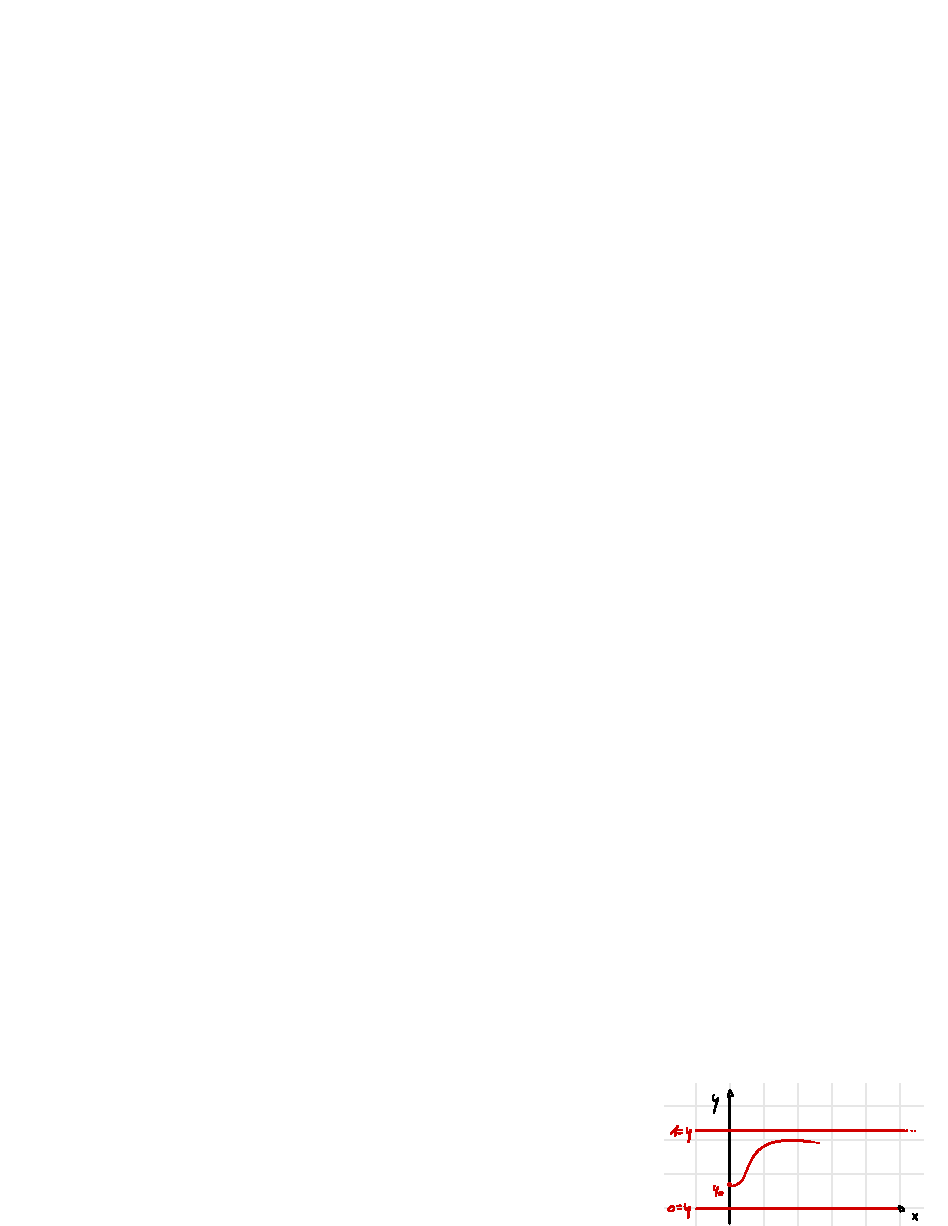
\includegraphics[width=0.7\textwidth]{img/modello_crescita_logaritmica-eg.pdf}
		\caption{Esempio di grafico con un certo $y_{0}$.}
	\end{figure}

	\newpage
	
	\subsection{Esercizio con domande da \textcolor{Red3}{esame}}
	
	Dato il seguente problema di Cauchy:
	
	\begin{equation*}
		\begin{cases}
			y^{'} = e^{x} + y^{2} \\
			y\left(0\right) = 1
		\end{cases}
	\end{equation*}

	\noindent
	Si \textbf{risponda alle seguenti \underline{domande}}:
	
	\begin{enumerate}[label=\Roman*]
		\item Scrivere l'equazione della tangente al grafico della curva con soluzione nel punto di coordinate $\left(0, 1\right)$.
		
		\item Vicino (o intorno) al punto $x = 0$, la funzione è concava o convessa?
	\end{enumerate}
	
	\noindent
	\textcolor{Green4}{\textbf{\underline{Risposta domanda I.}}}\newline
	
	\noindent
	L'equazione generale (o definizione) della retta tangente è:
	
	\begin{equation*}
		y - y_{0} = m \left(x - x_{0}\right)
	\end{equation*}

	\noindent
	Con $x_{0}$, $y_{0}$ che sono coordinate del punto $m$, ovvero la \emph{pendenza}. Quindi, andando a sostituire le coordinate fornite dall'esercizio nella definizione di retta tangente:
	
	\begin{equation*}
		\textbf{Sostituzione } \left(0, 1\right) \rightarrow y - 1 = m \left(x - 0\right)
	\end{equation*}

	\noindent
	Sapendo che la pendenza $m$ è la derivata della funzione calcolata nel punto zero, si eseguono questi calcoli usando la funzione fornita dall'esercizio:
	
	\begin{equation*}
		m \longrightarrow y^{'}\left(0\right) = e^{0} + \left[y\left(0\right)\right]^{2}; \hspace{2em} y^{'}\left(0\right) = 1 + 1^{2} = 2
	\end{equation*}

	\noindent
	Il valore noto viene sostituito nella definizione di retta tangente, quindi l'equazione di quest'ultima diventa:
	
	\begin{equation*}
		y - 1 = 2\left(x - 0\right) \longrightarrow y = 2x - 1
	\end{equation*}\newline
	
	\noindent
	\textcolor{Green4}{\textbf{\underline{Risposta domanda II.}}}\newline
	
	\noindent
	Per la concavità o convessità si studia la derivata seconda:
	
	\begin{equation*}
		y^{''}\left(x\right) = e^{x} + 2y\left(x\right) \cdot y^{'}\left(x\right)
	\end{equation*}

	\noindent
	Dalla derivata seconda ottenuta si inserisce la condizione del problema:
	
	\begin{equation*}
		y^{''}\left(0\right) = 1 + 2 \cdot 1 \cdot \textcolor{Red3}{2} = 5
	\end{equation*}

	\noindent
	Il \textcolor{Red3}{2} è il risultato della $y^{'}\left(0\right)$ trovato prima.
	
	Dato che il \textbf{\underline{risultato è positivo, allora la funzione è convessa}}. Più formalmente, in un intorno di $x = 0$, se la $y^{''}\left(0\right) > 0$, la funzione si dice che è convessa.
	
	\section{Lezione 03}
	
	\subsection{Equazioni differenziali del primo ordine}
	
	La forma generale di un'equazione differenziale lineare del \textbf{\underline{primo ordine}} è la seguente:
	
	\begin{equation*}
		y^{'} + a\left(x\right) y = f\left(x\right) \hspace{2em} \text{con } a\left(x\right), f\left(x\right) \in \mathcal{C}^{0}\left(I\right)
	\end{equation*}

	\noindent
	Si ricorda che la $I$ indica l'intervallo nell'insieme dei numeri naturali $\mathbb{R}$. Inoltre, l'\textbf{equazione} si dice:
	
	\begin{itemize}
		\item \textcolor{Red3}{\textbf{\underline{Omogenea}}}, se $f\left(x\right) \equiv 0$, cioè è nulla;
		\item \textcolor{Red3}{\textbf{\underline{Non omogenea}}}, se $f\left(x\right) \not\equiv 0$, cioè non nulla;
	\end{itemize}

	\noindent
	La \textbf{\underline{risoluzione}} di queste equazioni prevede due passaggi:
	
	\begin{enumerate}
		\item Determinare una primitiva $A\left(x\right)$ di $a\left(x\right)$ sull'intervallo dei reali $I$ e considerare la funzione $e^{A\left(x\right)}$;
		
		\item Moltiplicare entrambi i membri dell'equazione differenziale per $e^{A\left(x\right)}$, chiamato anche \textcolor{Red3}{\textbf{\underline{fattore integrante}}}.
	\end{enumerate}

	\noindent
	L'\textcolor{Red3}{\textbf{\underline{obbiettivo}}} finale, ovvero successivamente alla risoluzione, è avere al primo membro la derivata di un prodotto tra funzioni.\newline
	
	\noindent
	Più esplicitamente, in maniera \textbf{generalistica}, si eseguono i seguenti passaggi:
	
	\begin{enumerate}
		\item $\overbrace{e^{A\left(x\right)} \cdot y^{'}\left(x\right) + e^{A\left(x\right)} \cdot a\left(x\right) \cdot y\left(x\right)}^{\text{Derivata di un prodotto tra due funzioni}} = e^{A\left(x\right)} \cdot f\left(x\right) \hspace{2em} \forall x \in I$

		\item $e^{A\left(x\right)} \cdot y\left(x\right) = \int e^{A\left(x\right)} f\left(x\right) \: \mathrm{d}x \hspace{2em} \text{con } c \in \mathbb{R}$
	\end{enumerate}

	\noindent
	Per derivata di un prodotto tra due funzioni ovviamente si intende:
	
	\begin{equation*}
		\left(e^{A\left(x\right)} \cdot y\left(x\right)\right)^{'}
	\end{equation*}

	La \textcolor{Red3}{\textbf{\underline{forma risolutiva generale}}} è la seguente:
	
	\begin{equation*}
		y\left(x\right) = e^{-A\left(x\right)} \left(\int e^{A\left(x\right)} f\left(x\right) \: \mathrm{d}x + c\right)
	\end{equation*}

	\noindent
	Ovviamente, per determinare la costante $c$ si utilizzano le condizioni iniziali.
	
	\newpage
	
	\noindent
	Combinando l'equazione differenziale lineare del primo ordine con le condizioni iniziali, il sistema da risolvere è il di nuovo il \textcolor{Red3}{\textbf{\underline{problema di Cauchy}}}:
	
	\begin{equation*}
		\begin{cases}
			y^{'}\left(x\right) + a\left(x\right) \cdot y\left(x\right) = f\left(x\right)	& a\left(x\right), f\left(x\right) \in \mathcal{C}^{0}\left(I\right) \\
			y\left(x_{0}\right) = y_{0}														& x_{0}, y_{0} \in I
		\end{cases}
	\end{equation*}

	\noindent
	E per definizione del teorema dell'esistenza e dell'unicità (teoremi \ref{teorema esistenza} e \ref{teorema unicità} a pagina \pageref{teorema esistenza}), l'equazione differenziale lineare del primo ordine \textbf{\underline{ammette un'unica soluzione}} \textbf{\underline{di classe}} $\mathcal{C}^{1}\left(I\right)$. Si osservi che la soluzione è definita su \emph{tutto} l'intervallo e di conseguenza è una \textbf{\underline{soluzione globale}}!\newline
	
	\noindent
	Nei prossimi paragrafi vengono presentati degli esempi guidati.
	
	\newpage
	
	\subsubsection[Esempio 1]{\textcolor{Green4}{\textbf{Esempio 1}}}
	
	L'equazione differenziale è la seguente:
	
	\begin{equation*}
		y^{'} + 2xy = x
	\end{equation*}

	\noindent
	Si osservi che l'equazione differenziale, oltre ad essere risolvibile tramite la tecnica presentata nel paragrafo precedente, è possibile risolverla anche a \emph{variabili separabili} (paragrafo \ref{Equazioni a variabili separabili}). In quest'ultimo caso, l'equazione sarebbe:
	
	\begin{equation*}
		y^{'} = x\left(1-2y\right)
	\end{equation*}

	\noindent
	Tuttavia, si ricerca l'integrale generale come spiegato nel metodo nel paragrafo precedente.\newline
	
	\noindent
	\textcolor{Red3}{\textbf{\underline{Passo 1}}}\newline
	
	\noindent
	Data la  forma generale dell'equazione differenziale lineare del primo ordine:
	
	\begin{equation*}
		y^{'} + a\left(x\right) y = f\left(x\right)
	\end{equation*}

	\noindent
	Dall'equazione dell'esercizio si ottiene:
	
	\begin{equation*}
		\begin{array}{lll}
			y^{'} + 2xy = x & \longrightarrow	& a\left(x\right) = 2x \\
							& \longrightarrow	& f\left(x\right) = x
		\end{array}
	\end{equation*}

	\noindent
	Con entrambe le funzioni $a\left(x\right)$ e $f\left(x\right)$ continue sull'insieme dei reali $\mathbb{R}$.\newline
	
	\noindent
	\textcolor{Red3}{\textbf{\underline{Passo 2}}}\newline
	
	\noindent
	Si calcola la primitiva del fattore $a\left(x\right)$:
	
	\begin{equation*}
		a\left(x\right) = 2x \xrightarrow{\text{primitiva}} A\left(x\right) = x^{2}
	\end{equation*}

	\noindent
	Così da costruire la funzione $e^{A\left(x\right)}$:
	
	\begin{equation*}
		e^{A\left(x\right)} \xrightarrow{\text{sostituzione}} e^{x^{2}}
	\end{equation*}

	\noindent
	Funzione chiamata anche \textbf{\underline{fattore integrante}}.\newline
	
	\noindent
	\textcolor{Red3}{\textbf{\underline{Passo 3}}}\newline
	
	\noindent
	Grazie al passo precedente si ha il fattore integrante, il quale viene usato per moltiplicare entrambi i membri dell'equazione differenziale. Quindi:
	
	\begin{equation*}
		\begin{array}{lllll}
			\text{Equazione differenziale}					& \longrightarrow & y^{'} + 2x \: y = x && \forall x \in \mathbb{R}\\
			\text{Equazione diff. per } e^{A\left(x\right)}	& \longrightarrow & \underbrace{e^{x^{2}} \cdot y^{'} + e^{x^{2}} \cdot 2x \: y}_{\left(e^{x^{2}} y\left(x\right)\right)^{'}} = e^{x^{2}} \cdot x && \forall x \in \mathbb{R}
		\end{array}
	\end{equation*}

	\newpage
	
	\noindent
	\textcolor{Red3}{\textbf{\underline{Passo 4}}}\newline
	
	\noindent
	Data la \textbf{\emph{forma risolutiva generale}} delle equazioni differenziali lineari del primo ordine:
	
	\begin{equation*}\label{eq}
		y\left(x\right) = e^{-A\left(x\right)} \left(\int e^{A\left(x\right)} f\left(x\right) \: \mathrm{d}x + c\right)
	\end{equation*}
	
	\noindent
	Si sostituiscono i valori noti e si calcola l'integrale:
	
	\begin{equation*}
		\begin{array}{lll}
			\text{Forma risolutiva generale}					& \longrightarrow & \text{(equazione sopra)} \\
			&& \\
			\text{Forma risolutiva generale con valori noti}	& \longrightarrow & e^{x^{2}} \cdot y\left(x\right) = \displaystyle \int x \cdot e^{x^{2}} \: \mathrm{d}x + c \\
			&& \\
																& \hookrightarrow & e^{x^{2}} \cdot y\left(x\right) = \dfrac{e^{x^{2}}}{2} + c \\
			&& \\
			\textbf{Integrale generale (forma finale)}			& \hookrightarrow & y\left(x\right) = \dfrac{1}{2} + c e^{-x^{2}}
		\end{array}
	\end{equation*}

	\noindent
	L'integrale generale ha sempre la $x$ nell'insieme dei reali ovviamente $x \in \mathbb{R}$.
	
	\newpage
	
	\subsubsection[Esempio 2]{\textcolor{Green4}{\textbf{Esempio 2}}}
	
	L'equazione differenziale è la seguente:
	
	\begin{equation*}
		y^{'} - \dfrac{1}{t} y = t^{2}
	\end{equation*}

	\noindent
	Si ricerca l'integrale generale.\newline
	
	\noindent
	\textcolor{Red3}{\textbf{\underline{Passo 1}}}\newline
	
	\noindent
	Data la forma generale dell'equazione differenziale lineare del primo ordine:
	
	\begin{equation*}
		y^{'} + a\left(x\right) y = f\left(x\right)
	\end{equation*}
	
	\noindent
	Si evidenziano i termini $a\left(x\right)$ e $f\left(x\right)$ nell'equazione differenziale dell'esercizio:
	
	\begin{equation*}
		\begin{array}{lll}
			y^{'} - \dfrac{1}{t} y = t^{2}	& \longrightarrow & a\left(t\right) = - \dfrac{1}{t} \\
											& \longrightarrow & f\left(t\right) = t^{2}
		\end{array}
	\end{equation*}

	\begin{center}
		\noindent
		\textcolor{Blue3}{\textbf{\underline{Attenzione!}}}
	\end{center}
	Si noti bene che in questo caso la $a\left(t\right)$ è definita nell'insieme: $\left(0, +\infty\right)$. Questo perché la funzione è una frazione e sicuramente non può essere una $0$. Inoltre, dato che \textbf{il problema di Cauchy si definisce solo su intervalli} e nel nostro caso la frazione sarebbe l'unione di due intervalli escluso lo $0$, cioè $\left(-\infty, 0\right) \cup \left(0, +\infty\right)$, è necessario scegliere quale intervallo utilizzare. La decisione viene presa in base ad una specifica dell'esercizio oppure, più frequentemente, in base al punto iniziale fornito dal problema di Cauchy. Infatti, se il punto iniziale fosse maggiore di $0$, si sceglierebbe l'intervallo $\left(0, +\infty\right)$, altrimenti, se fosse negativo, si sceglierebbe l'intervallo $\left(-\infty, 0\right)$.\newline
	
	\noindent
	Al contrario, la funzione $f\left(t\right)$ è definita nell'insieme dei reali $\mathbb{R}$.\newline
	
	\noindent
	\textcolor{Red3}{\textbf{\underline{Passo 2}}}\newline
	
	\noindent
	Si calcola la primitiva di $a\left(t\right)$ per costruire il fattore integrante. Quindi:
	
	\begin{equation*}
		a\left(t\right) = - \dfrac{1}{t} \xrightarrow{\text{primitiva}} A\left(t\right) = -\ln t
	\end{equation*}

	\noindent
	E di conseguenza il fattore integrante corrisponde a $e^{-\ln t}$. Con qualche accorgimento è possibile riscrivere il fattore integrante come:
	
	\begin{equation*}
		e^{-\ln t} = \dfrac{1}{t}
	\end{equation*}

	\noindent
	Il meno scompare perché si utilizza la proprietà fondamentale dei logaritmi e si ottiene $t^{-1}$.
	
	\newpage
	
	\noindent
	\textcolor{Red3}{\textbf{\underline{Passo 3}}}\newline
	
	\noindent
	Si esegue la moltiplicazione del fattore integrante per l'equazione differenziale:
	
	\begin{equation*}
		\begin{array}{lllll}
			\text{Equazione differenziale}					& \longrightarrow & y^{'} - \dfrac{1}{t} y = t^{2} && \\
			&&&& \\
			\text{Equazione diff. per } e^{A\left(x\right)}	& \longrightarrow & \underbrace{\dfrac{1}{t}y^{'} - \dfrac{1}{t^{2}}}_{\left(\dfrac{1}{t}y\left(t\right)\right)^{'}} = t && \text{con } t \in \left(0, +\infty\right)
		\end{array}
	\end{equation*}

	\noindent
	L'insieme in cui cade $t$ è definito nello stesso modo del passo 1.\newline

	\noindent
	\textcolor{Red3}{\textbf{\underline{Passo 4}}}\newline
	
	\noindent
	L'esercizio si conclude calcolando l'integrale generale tramite l'integrale vero e proprio:
	
	\begin{equation*}
		\begin{array}{rll}
			\dfrac{1}{t}y				& = &	\displaystyle\int t \: \mathrm{d}t + c \\
			&& \\
										& = &	\dfrac{1}{t}y = \dfrac{t^{2}}{2} + c \\
			&& \\
			\textbf{Integrale generale}	& = &	y\left(t\right) = \dfrac{1}{2} t^{3} + ct
		\end{array}
	\end{equation*}

	\noindent
	Con $t$ definita nell'insieme del passo 1, cioè $t \in \left(0, +\infty\right)$. Al contrario, la costante $c$ in tutto l'insieme dei reali, quindi $c \in \mathbb{R}$.
	
	\newpage
	
	\subsubsection[Esempio 3]{\textcolor{Green4}{\textbf{Esempio 3}}}
	
	L'equazione differenziale è la seguente:
	
	\begin{equation*}
		x^{'}\left(t\right) + \cot \left(t\right) x\left(t\right) = e^{t}
	\end{equation*}

	Si ricerca l'integrale generale.\newline
	
	\noindent
	\textcolor{Red3}{\textbf{\underline{Passo 1}}}\newline
	
	\noindent
	Talvolta le equazioni differenziali hanno variabili diverse dal solito, ma il ragionamento rimane invariato. In questo caso, l'equazione ha la variabile $t$ definita nell'intervallo $t \in \left(0, \pi\right)$. Il motivo è banale:
	
	\begin{equation*}
		\cot\left(t\right) = \dfrac{\cos\left(t\right)}{\sin\left(t\right)}
	\end{equation*}

	\noindent
	Data la forma generale dell'equazione differenziale lineare di primo grado:
	
	\begin{equation*}
		y^{'} + a\left(x\right) y = f\left(x\right)
	\end{equation*}

	\noindent
	Si evidenziano i termini $a\left(t\right)$ e $f\left(t\right)$ dall'equazione:
	
	\begin{equation*}
		\begin{array}{lll}
			x^{'}\left(t\right) + \cot \left(t\right) x\left(t\right) = e^{t}	& \longrightarrow & a\left(t\right) = \cot\left(t\right) \\
			& \longrightarrow & f\left(t\right) = e^{t}
		\end{array}
	\end{equation*}

	\noindent
	\textcolor{Red3}{\textbf{\underline{Passo 2}}}\newline
	
	\noindent
	Si calcola la primitiva di $a\left(t\right)$ così da ottenere il fattore integrante. Quindi:
	
	\begin{equation*}
		a\left(t\right) = \cot\left(t\right) \xrightarrow{\text{primitiva}} A\left(t\right) = \int\dfrac{\cos\left(t\right)}{\sin\left(t\right)} \: \mathrm{d}t = \ln \left|sin\left(t\right)\right|
	\end{equation*}
	
	\noindent
	Si sostituisce la primitiva nella definizione del fattore integrante $e^{A\left(t\right)}$ e si ottiene:
	
	\begin{equation*}
		e^{A\left(t\right)} \xrightarrow{\text{sostituzione}} e^{\ln\left|\sin\left(t\right)\right|} = \left|\sin\left(t\right)\right| = \sin\left(t\right)
	\end{equation*}
	
	\noindent
	È possibile portare il $\sin$ fuori dall'esponente grazie ad una delle proprietà dei logaritmi. Inoltre, grazie alla definizione dell'insieme in cui è definita $t$, cioè $t\in\left(0, +\infty\right)$, è possibile anche rimuovere il valore assoluto dato che sarà sempre positivo.\newline
	
	\noindent
	\textcolor{Red3}{\textbf{\underline{Passo 3}}}\newline
	
	\noindent
	L'equazione differenziale trovata al passo precedente viene moltiplicata per il fattore integrante:
	
	\begin{equation*}
		\begin{array}{lll}
			\text{Equazione differenziale}					& \longrightarrow & x^{'}\left(t\right) + \cot \left(t\right) x\left(t\right) = e^{t} \\
			&& \\
			\text{Equazione diff. per } e^{A\left(t\right)}	& \longrightarrow & \underbrace{\sin\left(t\right) \cdot x^{'}\left(t\right) + \cos\left(t\right) x\left(t\right)}_{\left(x\left(t\right) \cdot \sin\left(t\right)\right)^{'}} = e^{t} \cdot \sin\left(t\right)
		\end{array}
	\end{equation*}

	\noindent
	Il termine $\cos$ si ricava dall'operazione di moltiplicazione tra cotangente $\cot = \dfrac{\cos\left(t\right)}{\sin\left(t\right)}$ e il seno $\sin\left(t\right)$ che rappresenta il fattore integrante.
	
	\newpage
	
	\noindent
	\textcolor{Red3}{\textbf{\underline{Passo 4}}}\newline
	
	\noindent
	Si conclude l'esercizio trovando l'integrale generale:
	
	\begin{equation*}
		\begin{array}{lll}
			x\left(t\right) \cdot \sin\left(t\right) 	& = & \displaystyle\int e^{t} \sin\left(t\right) \: \mathrm{d}t \\
			&& \\
			\text{Integrale per parti}					& = & e^{t} \sin\left(t\right) - \displaystyle\int e^{t} \cos\left(t\right) \: \mathrm{d}t \\
			&& \\
			\text{Si ripete integrazione per parti}		& = & e^{t} \sin\left(t\right) - \left(e^{t} \cos\left(t\right) + \displaystyle\int e^{t} \sin\left(t\right) \: \mathrm{d}t \right) \\
			&& \\
														& = & e^{t} \sin\left(t\right) - e^{t} \cos\left(t\right) - \displaystyle\int e^{t} \sin\left(t\right) \: \mathrm{d}t
		\end{array}
	\end{equation*}

	\noindent
	Dato che l'incognita iniziale era l'integrale $\int e^{t} \sin\left(t\right) \: \mathrm{d}t$ e il risultato che è stato trovato corrisponde a $e^{t} \sin\left(t\right) - e^{t} \cos\left(t\right) - \displaystyle\int e^{t} \sin\left(t\right) \: \mathrm{d}t$, è possibile eguagliare questi due termini per ottenere la soluzione dell'integrale:
	
	\begin{equation*}
		\begin{array}{lll}
			\displaystyle\int e^{t} \sin\left(t\right) \: \mathrm{d}t	& = & e^{t} \sin\left(t\right) - e^{t} \cos\left(t\right) - \displaystyle\int e^{t} \sin\left(t\right) \: \mathrm{d}t \\
			&& \\
			\displaystyle\int e^{t} \sin\left(t\right) \: \mathrm{d}t + \displaystyle\int e^{t} \sin\left(t\right) \: \mathrm{d}t	& = & e^{t} \sin\left(t\right) - e^{t} \cos\left(t\right) \\
			&& \\
			2 \cdot \displaystyle\int e^{t} \sin\left(t\right) \: \mathrm{d}t & = & e^{t} \sin\left(t\right) - e^{t} \cos\left(t\right) \\
			&& \\
			\displaystyle\int e^{t} \sin\left(t\right) \: \mathrm{d}t 	& = & \dfrac{e^{t} \sin\left(t\right) - e^{t} \cos\left(t\right)}{2} \\
			&& \\
			\displaystyle\int e^{t} \sin\left(t\right) \: \mathrm{d}t 	& = & \dfrac{1}{2} \cdot e^{t} \left(\sin\left(t\right) - \cos\left(t\right)\right) + c
		\end{array}
	\end{equation*}

	\noindent
	Per concludere, si riprendere l'equazione generale iniziale e si sostituisce il risultato dell'integrale trovato:
	
	\begin{equation*}
		x\left(t\right) \cdot \sin\left(t\right) = \dfrac{1}{2} \cdot e^{t} \left(\sin\left(t\right) - \cos\left(t\right)\right) + c
	\end{equation*}

	\noindent
	Si esplicita l'incognita e si ottiene l'\textbf{integrale generale}:
	
	\begin{equation*}
		x\left(t\right) = \dfrac{1}{2} \cdot e^{t} \cdot \left(1 - \cot\left(t\right)\right) + \dfrac{c}{\sin\left(t\right)}
	\end{equation*}

	\newpage
	
	\subsection{Operatore differenziale lineare}
	
	Con un punto di vista ancora più generale, si definisce una particolare applicazione che si posiziona tra lo spazio continuo $\mathcal{C}^{1}\left(I\right)$ delle funzioni con derivata continua sull'intervallo $I$ e lo spazio continuo $\mathcal{C}^{0}\left(I\right)$ delle funzioni continue su $I$:
	
	\begin{equation}\label{operatore differenziale lineare di ordine 1}
		\begin{array}{llllll}
			L:	& \mathcal{C}^{1}\left(I\right) & \longrightarrow & \mathcal{C}^{0}\left(I\right) && \\
				& y\left(x\right)				& \longmapsto 	  & y^{'}\left(x\right) + a\left(x\right)y\left(x\right) && \text{con } a\left(x\right) \text{continua su } I
		\end{array}
	\end{equation}

	\noindent
	L'operazione definita e rappresentata dalla lettera $L$ si chiama: \textcolor{Red3}{\textbf{\underline{operatore}}} \textcolor{Red3}{\textbf{\underline{differenziale lineare di ordine 1}}}. Anche per questa operazione vale la \textbf{linearità}.\newline

	\noindent\fbox{%
		\parbox{\textwidth}{%
			\begin{center}
				\textcolor{Red3}{\textbf{\underline{Linearità}}}
			\end{center}
			
			\noindent
			Se $y_{1}\left(x\right), y_{2}\left(x\right) \in \mathcal{C}^{1}\left(I\right)$, allora l'operatore differenziale lineare di ordine 1 viene moltiplicato considerando anche le costanti:
			
			\begin{equation*}
				L\left(\alpha y_{1}\left(x\right) + \beta y_{2}\left(x\right)\right) = \alpha L\left(y_{1}\left(x\right)\right) + \beta L\left(y_{2}\left(x\right)\right) \hspace{2em} \text{con } \alpha, \beta \in \mathbb{R}
			\end{equation*}
			
			\noindent
			Quindi, l'equazione differenziale con la sua forma classica $y^{'}\left(x\right) + a\left(x\right) y\left(x\right) = f\left(x\right)$ con la funzione $f\left(x\right)$ continua sull'intervallo $I$, si può anche riscrivere come:
			
			\begin{equation*}
				L\left(y\left(x\right)\right) = f\left(x\right)
			\end{equation*}
		}%
	}

	\vspace{1.5em}

	\noindent
	Da questa definizione di linearità, la \textcolor{Red3}{\textbf{\underline{soluzione}}} cambia a seconda del tipo:
	
	\begin{itemize}[label=\ding{42}]
		\item \textcolor{Red3}{\textbf{\underline{Omogenea.}}} Allora la funzione $f\left(x\right) = 0$ e di conseguenza l'equazione differenziale $L\left(y\left(x\right)\right) = 0$ ovvero:
		\begin{equation*}
			v = \ker\left(L\right) \text{ è sottospazio vettoriale di } \mathcal{C}^{1}\left(I\right)
		\end{equation*}
		Dove:
		\begin{itemize}[label=-]
			\item $v$ rappresenta l'\textbf{insieme delle soluzioni} dell'omogenea associata;			
			\item $\ker\left(L\right)$ è il \textbf{nucleo} (\emph{kernel}, $\ker$) dell'\textbf{applicazione lineare} $L$;
			\item Il sottospazio vettoriale è chiaro, ma si ricordi che nel caso di equazioni differenziali del primo ordine, la \textbf{dimensione del sottospazio è pari a} $1$.
		\end{itemize}
		L'\textbf{\underline{obbiettivo}} delle soluzioni omogenee è trovare le funzioni di classe $\mathcal{C}^{1}$ che hanno come immagine un vettore nullo.
		
		\item \textcolor{Red3}{\textbf{\underline{Non omogenea.}}} L'insieme delle soluzioni dell'equazione differenziale $L\left(y\left(x\right)\right) = f\left(x\right)$ è definita come:
		\begin{equation*}
			\left\{y_{p}\left(x\right) + y_{v}\left(x\right) : y_{v}\left(x\right) \in \ker\left(L\right)\right\}
		\end{equation*}
	\end{itemize}
\end{document}